\documentclass[a4paper]{article}

\usepackage[utf8]{inputenc}  
\usepackage[francais]{babel}  
\usepackage[top=2cm, bottom=2cm, left=2cm, right=2cm]{geometry}
\usepackage{graphicx}

\begin{document}

\begin{titlepage}
	~ 
	\vfill
	\begin{center}
		\begin{Huge}
			Projet Administration Réseau : \\ Étude d'architecture\\
		\end{Huge}
	\vfill
		\textbf{Hexanôme 4211 :} 
			\\Sandra \bsc{Mondain}, Elisa \bsc{Abidh}, 
			\\Gaël \bsc{Motte}, Armand \bsc{Rossius}, 
			\\Nicolas \bsc{Silva}, Julien \bsc{Levesy}\\
	\vfill
	\end{center}
	\vfill
\end{titlepage}

%\newpage
%\tableofcontents
\newpage


	\section{Description} % redétailler en séparant interconnexion et sur chaque site. mettre en avant la sécurité. 	
	
	Afin de mettre en place une communication sécurisée entre les différents sites, nous optons pour une solution basée sur un VPN (Virtual Private Network). 
	
	\paragraph*{} % Routeurs VPN
	L'utilisation du VPN ne concernant que les machines et les automates de l'AIP, nous plaçons sur chaque site de l'AIP un routeur équipé d'un client VPN qui fait la passerelle entre le site et le réseau du campus. Ces routeurs VPN sont également équipés de firewalls. 
	
	\paragraph*{} % Switchs VLAN
	%Comme les automates peuvent être situés dans différentes salles sur chaque site, on mettra en place un sous-réseau par salle, en utilisant des switchs VLAN (Virtual Local Area Network). L'utilisation de ces switchs permet également de limiter le broadcast UDP des automates sur le réseau. 
	Chaque site peut contenir des automates et des PC de travail. On mettra en place un sous-réseau comprenant tous les automates et un autre sous-réseau comprenant tous les PC, en utilisant des switchs VLAN (Virtual Local Area Network). L'utilisation de ces switchs permet de limiter le broadcast UDP des automates sur le réseau. 
	
	\paragraph*{} % DNS 
	Nous allons mettre en place un serveur DNS par site. Ceci permettra de déplacer des plate-formes mobiles d'un site à un autre, car l'utilisation des DNS originaux des campus poserait un problème de réactivité pour la création ou suppression d'une entrée. 
	
	\paragraph*{} % DHCP
	Nous mettrons également en place un serveur DHCP par site pour gérer dynamiquement l'adressage des parcs de machines et d'automates de l'AIP. 
	
	\paragraph*{} % Authentification et Annuaires LDAP
	L'authentification sur site se fera au moyen d'un groupe d'utilisateur répliqué sur tous les annuaires LDAP des différents campus. Ainsi, les utilisateurs mobiles d'un site AIP à l'autre pourront s'authentifier où qu'ils soient. L'authentification depuis l'extérieur pourra se faire grâce à un client VPN déployé sur une machine distante, avec une politique d'authentification par certificat. 
	
	
	\newpage
	
	
	\section{Schéma de l'architecture}
	Sur le schéma ci-dessous, on peut voir les différents éléments qui constitueront le réseau. Le tunnel VPN ainsi créé est représenté en rouge. \\
	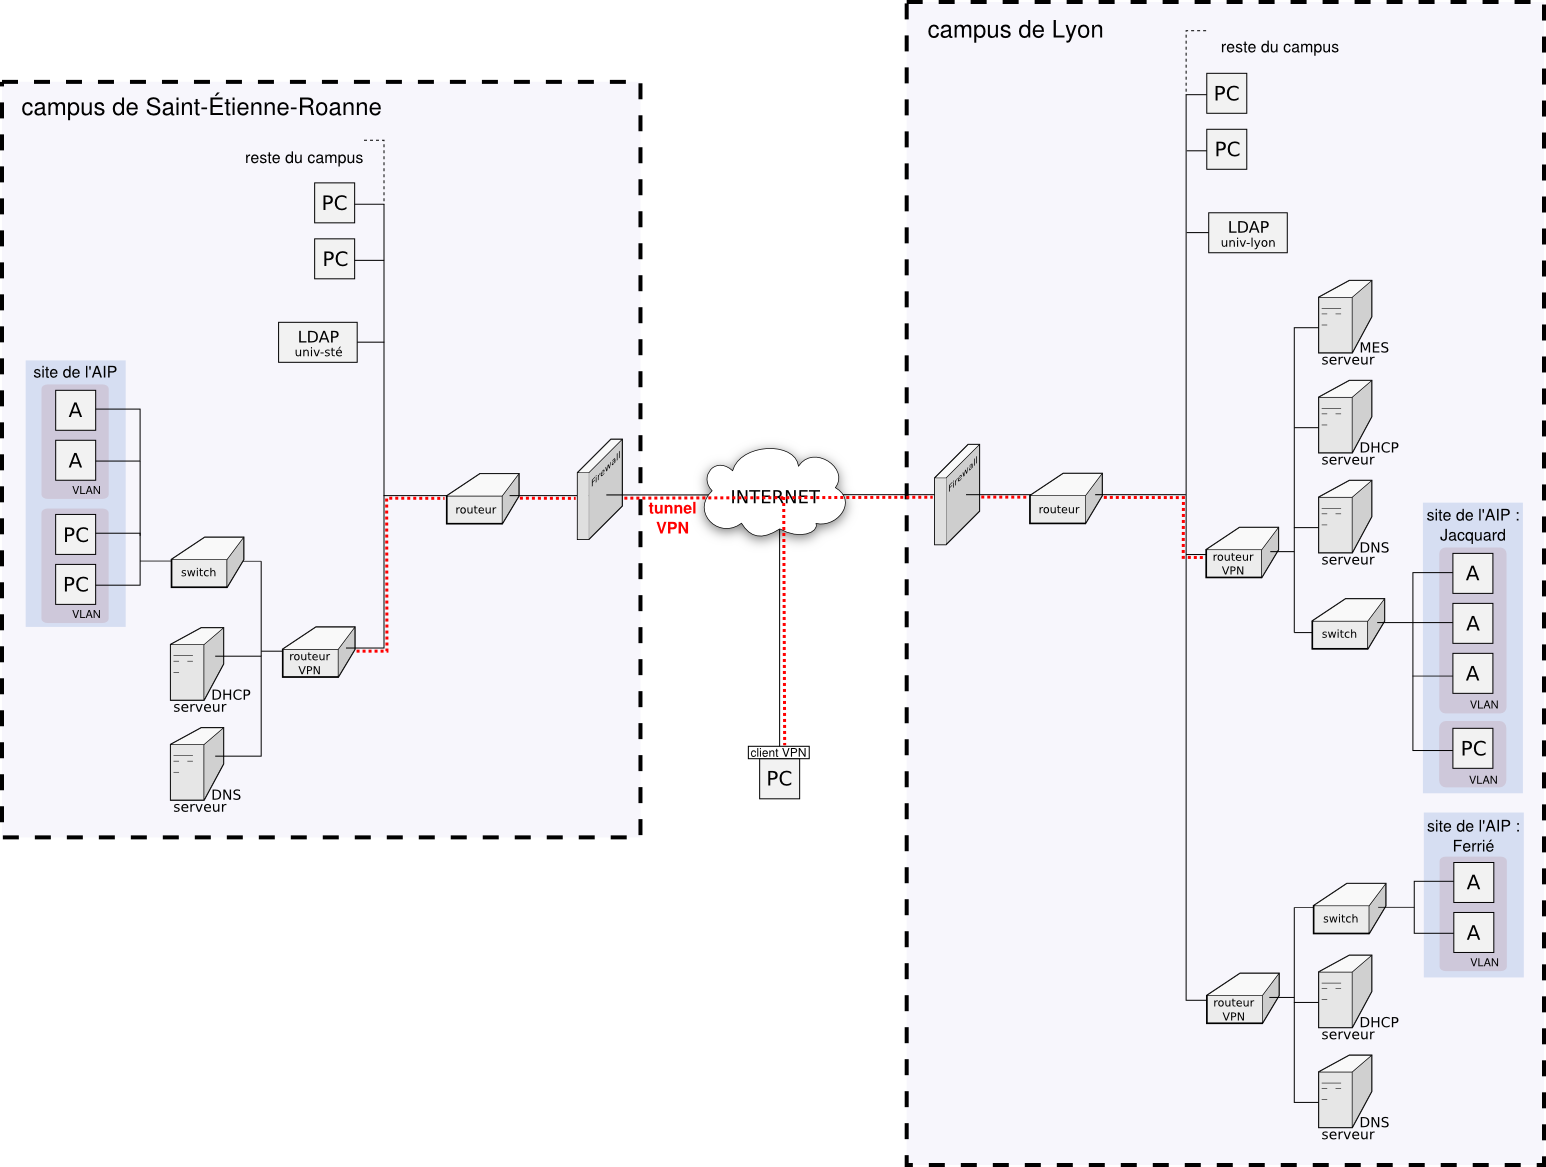
\includegraphics[width=\linewidth]{schema_archi.png}

\section{Spécification détaillée de l'architecture}
	\subsection{Définition des matériels}
	L'installation vise à s'insérer au mieux dans les réseaux existants. Cependant quelques matériels particulier devront être achetés.
	\subsubsection{Routeurs VPN}
Ils sont à la base de l'architecture et sont situés à l'entrée de chacun des sites de l'AIP.
Ils permettent les communications sécurisées site à site, mais également les communications vers un PC distant.
\paragraph{Matériel envisagé}
Le matériel proposé dans les documentations fournies peut convenir. En effet, il permet l'utilisation de VPN sur deux protocoles différents : 
\begin{itemize}
	\item{VPN de PPTP} Ce mode est intégré à Windows par l'utilisation de Radius.
	\item{VPN L2TP IPSEC} Ce mode de fonctionement ne propose pas d'outils de QoS ce qui empêche toute utilisation de ce mode pour la VoIP ou visioconférence.
\end{itemize}

	\subsubsection{Switchs VLAN}
Ces switchs permettent d'isoler les équipements qui peuvent inonder le réseau. Ainsi, les plateformes de TP qui utilisent le broadcast UDP peuvent être isolées dans un sous-réseau, tout en restant accessibles depuis l'extérieur.
	
	\subsubsection{Switchs conventionnels}
Ces switchs permettent juste de connecter l'ensemble des machines de l'AIP. Ils n'ont aucune intelligence propre.
	
	\subsubsection{Serveur DHCP}
Le serveur DHCP aura pour rôle l'attribution des adresses ip aux divers machines qui seront connectées. Les IP seront établies en fonctions du rôle et de la nature de la machine à connecter.

	\subsubsection{Dimensionnement}
Pour le dimensionement de ces équipements, nous nous limiterons à une gamme. En effet, les prestataire d'interventions dimensionnent eux-mêmes ces installation.\\
Au vue de la documentation fournie., plusieurs choix peuvent être faits : 
\begin{itemize}
	\item \textbf{Routeurs VPN} La Gamme S@n convient à l'utilisation VPN que l'on aura de ces routeurs.
	\item \textbf{Switchs VLAN} Nous utiliserons les VLAN proposés par Schneider Electric de la gamme ConneXium parametrables. 
	\item \textbf{Switchs conventionnels} Nous utiliseront ceux de la même gamme ConneXium non paramétrables cette fois ci. 
	\item \textbf{Serveurs DHCP} Cette fonctionnalité est très légère et ne nécessite pas d'infrastructure lourde. Le dimensionnement de cette machine ne sera pas abordé ici.
\end{itemize}
	
	
\end{document}
